%% TRANSFORMATIONS
%%

\subsection{Overview}

When plotted in the original $\mathbf{c}=\{c_2,c_3,c_4\}$ parameter space 
(Fig.~\ref{fig:c3Dplot}), the loci of physically allowed LDCs resembles a 
rotated, tilted ellipse of thin but finite width with a symmetric protrusion 
running along the semi-major axis. This complex morphology cannot be easily
sampled from and if one wished to draw a set of LDCs from a uniform prior, there
would be no alternative except to draw from the full cuboid and perform
an acceptance/rejection test using our seven analytic criteria. As evident from
Fig.~\ref{fig:c3Dplot}, the volume of allowed points is much less than the 
bounding cuboid volume, meaning that such a procedure would be highly 
inefficient. Numerical tests reveal that the efficiency of such a procedure is
just under 1\%, making any algorithms using this method very wasteful.

We are therefore motivated to try and transform the geometry of the accepted
loci of points into a more regular shape that we can sample from efficiently.
We previously did this in the 2D case of quadratic limb darkening in 
\citet{LD:2013}, but the transformative geometry required here is not only
more complex but also includes an extra dimension.

\subsection{Re-scaled LDCs}

We begin by noting that the envelope functions shown in 
Fig.~\ref{fig:c3c2surface}-\ref{fig:c4c3surface} provide an excellent 
description for the bounding region of allowed LDCs. Despite some small 
exceptions, we are motivated to exclusively use these simple envelopes 
rather than the full criteria since i) they provide a nearly perfect description 
of the loci ii) the envelopes are symmetric functions derived from quadratic 
forms iii) all of the envelopes come from criteria A and G alone. In practice, 
criterion F is also necessary to remove a duplicate set of solutions.

We therefore proceed to only consider the region contained by criteria A, F \& 
G, which we denote as the simplified region. This simplification means that the
bounding cuboid is slightly modified to:

\begin{align}
0 < c_2 < 9,\nonumber\\
-8-6\sqrt{2} < c_3 < -8+6\sqrt{2},\nonumber\\
0 < c_4 < 9.
\end{align}

As a first transformation, we re-scale the axes into a unitary cube by the use 
of $d_i$ terms, defined as:

\begin{align}
d_2 &= c_2/9, \nonumber\\
d_3 &= \frac{6\sqrt{2} - 8 - c_3}{12\sqrt{2}}, \nonumber\\
d_4 &= c_4/9.
\end{align}

\subsection{Righting the Allowed Region}

We next note that the loci (in $\mathbf{d}$ parameter space) resembles an
elliptic thin disk with the semi-major axis pointing along the unit vector 
$\{1,1,1\}$. Further, the disk appears rotated about this unit vector, with
respect to the axes of the reference frame. We decided to try to right the 
volume by performing a clockwise rotation of $(\pi/3)$\,radians about the unit 
vector ($\mathbf{M}_1$). We then perform a further rotation which re-locates the 
unit vector $\{1,1,1\}$ to $\{1,1,0\}$ ($\mathbf{M}_2$), followed by a third 
rotation re-locating $\{1,1,0\}$ to $\{1,0,0\}$ ($\mathbf{M}_3$). The total 
rotation matrix applied is described by:

\begin{align}
{\bf e} &= {\bf M_3}.{\bf M_2}.{\bf M_1}.{\bf d},\nonumber\\
{\bf e} &= {\bf M}.{\bf d},
\end{align}

where

\begin{eqnarray}
{\bf M} =\left(\begin{matrix}
\frac{1}{\sqrt{3}} & \frac{1}{\sqrt{3}} & \frac{1}{\sqrt{3}} \cr
-\frac{1}{\sqrt{2}} & 0 & \frac{1}{\sqrt{2}} \cr
\frac{1}{\sqrt{6}} & -\frac{\sqrt{2}}{\sqrt{3}} & \frac{1}{\sqrt{6}} \cr \end{matrix}\right).
\label{eqn:Mrot}
\end{eqnarray}

Applying these transformations gives a new-coordinate system of:

\begin{align}
e_2 &= \frac{ 36 - 24\sqrt{2} + 8c_2 - 3\sqrt{2}c_3 + 8c_4 }{ 72\sqrt{3} },\\
e_3 &= \frac{ c_4 - c_2 }{ 9\sqrt{2} },\\
e_4 &= \frac{ 24 - 18\sqrt{2} + 2\sqrt{2}c_2 + 3c_3 + 2\sqrt{2}c_4 }{ 36\sqrt{3} }.
\label{eqn:espace}
\end{align}

After visually inspecting the loci in this transformed parameter space (as
shown in Fig.~\ref{fig:e3Dplot}), we note that the allowed region now resembles 
a cone. Motivated by this observation, we proceed to transform this shape into a 
cone of symmetric proportions and with principal axes aligned to the transformed 
frame.

%%% 3D plot of the e-space
\begin{figure}
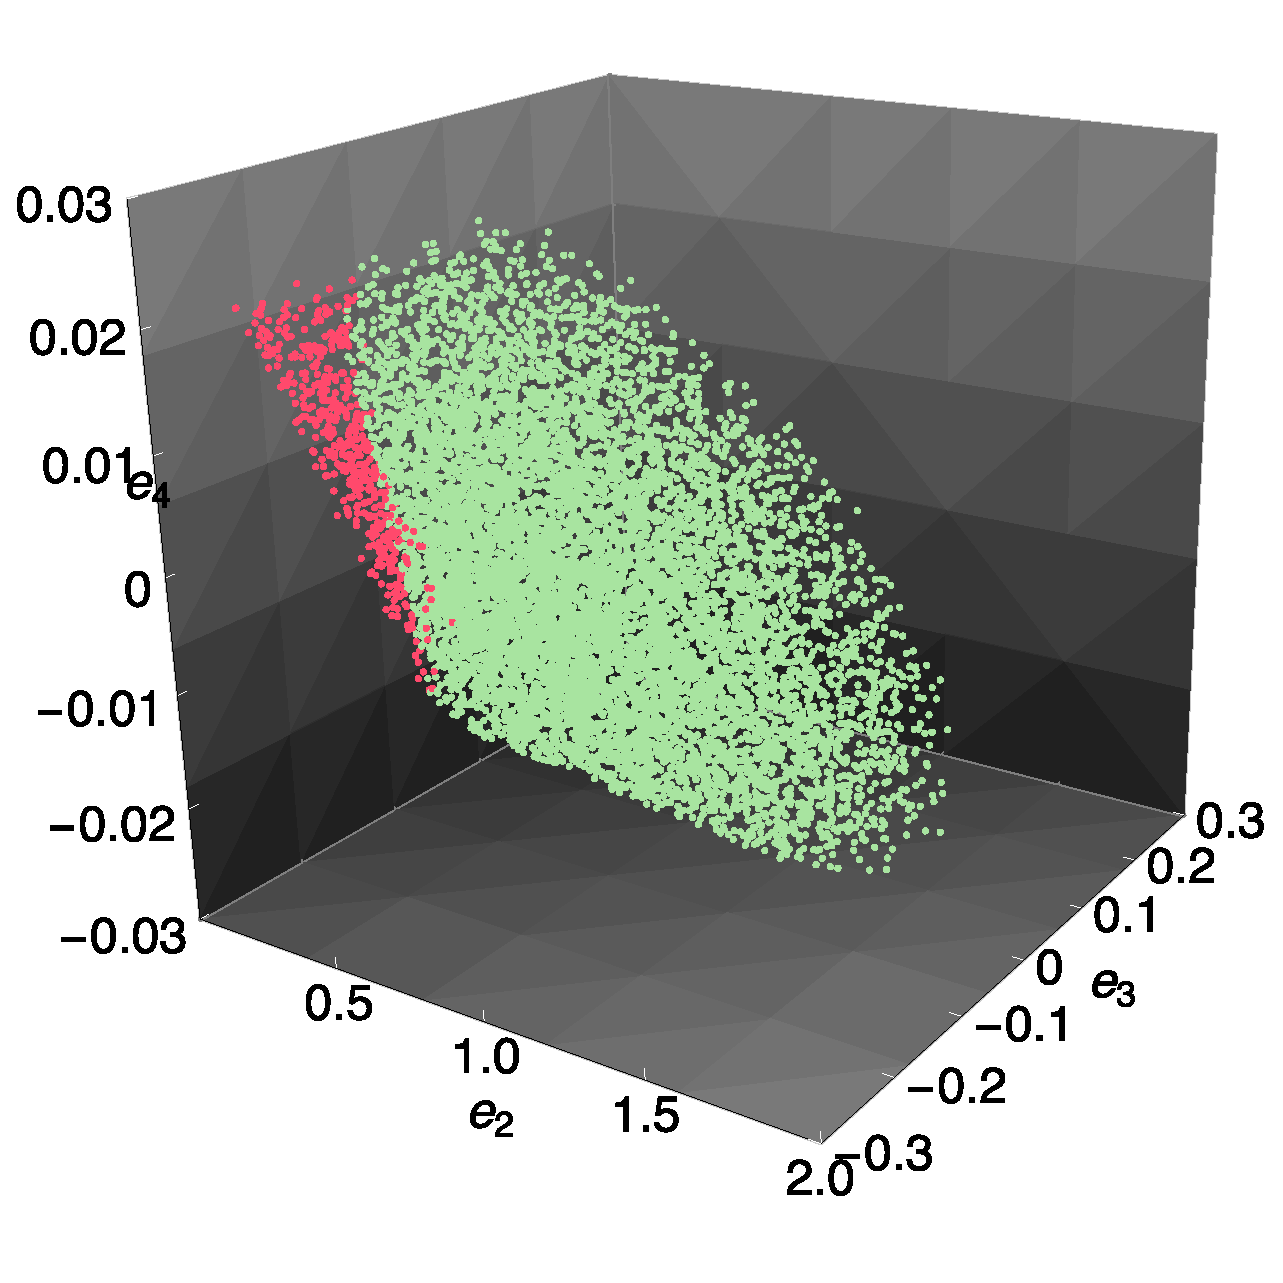
\includegraphics[width=\columnwidth]{e3Dplot.eps}
\caption{
Same as Fig.~\ref{fig:c3Dplot}, except the coordinates have been transformed
from $\{c_2,c_3,c_4\}\to\{e_2,e_3,e_4\}$. In this parameterization, we observe
that the volume of green points resembles a cone.
}
\label{fig:e3Dplot}
\end{figure}

\subsection{The Conal Region}

As with the $\mathbf{c}$ parameter space, our first step is to re-scale the
axis into a cuboid with unit lengths, requiring us to first compute the extrema
in $\mathbf{e}$ space.

The extrema of $e_3(c_2,c_4)$ occur when $(c_4-c_2)$ is maximized/minimized,
as evident from Equation~\ref{eqn:espace}. This can be considered further by 
studying our earlier illustration in Fig.~\ref{fig:c4c2surface}. This can be 
found by maximizing the function $(c_4^{\pm}-c_2)$ with respect to $c_2$, which 
reveals the extrema is $-3<(c_4-c_2)<+3$. We are therefore able to show that 
$-\frac{1}{3\sqrt{2}}<e_3<\frac{1}{3\sqrt{2}}$. This can also be achieved by
maximizing/minimizing the $e_3$ expression using the additional constraints of
criteria A, F \& G. Repeating for the other terms we define a new boundary box
of:

\begin{align}
\frac{ 3\sqrt{3} - 2\sqrt{6} }{ 18 } < &e_2 < \frac{ 2 (3+\sqrt{2}) }{ 3 \sqrt{3} },\\
-\Bigg(\frac{1}{3\sqrt{2}}\Bigg) < &e_3 < \Bigg(\frac{1}{3\sqrt{2}}\Bigg),\\
-\Bigg(\frac{ 3\sqrt{2} - 4 }{ 6\sqrt{3} }\Bigg) < &e_4 < \Bigg(\frac{ 3\sqrt{2} - 4 }{ 6\sqrt{3} }\Bigg).
\end{align}

We choose to re-scale the $e$-parameter space into a unit vector cube via:

\begin{align}
f_2 &= \frac{ e_2 - \frac{ 3\sqrt{3} - 2\sqrt{6} }{ 18 } }{ \frac{\sqrt{2}}{\sqrt{3}} + \frac{\sqrt{3}}{2} } ,\\
f_3 &= \frac{ 3 e_3 }{ \sqrt{2} },\\
f_4 &= \frac{ e_4 + \frac{ 3\sqrt{2} - 4 }{ 6\sqrt{3} } }{ \frac{ 6\sqrt{2} - 8 }{ 6\sqrt{3} } }.\\
\end{align}

At this point, we now choose to rotate the conic section by $\pi/4$ radians
in a clockwise sense around the $f_3$-axis, so that the cone's apex is located
at the origin and the cone points along the $e_3$-axis. We accomplish this using
an additional change of variables:

\begin{align}
g_2 &= \frac{f_2-f_4}{2},\\
g_3 &= f_3,\\
g_4 &= \frac{f_2+f_4}{\sqrt{2}},
\end{align}

where we have additionally normalized $g_2$ by a factor of $\sqrt{2}$ to allow
the loci to be symmetric on the $g_2$-$g_3$ plane.

In this frame, our cone now has an apex at zero, with a height of
$H = (\frac{10\sqrt{2}}{3} - 4)$ and a radius of $R = 1/\sqrt{2}$, as shown in
Fig.~\ref{fig:g3Dplot}. Writing out the $g$ terms relative to the original 
$c_i$ coefficients, we have:

\begin{align}
g_2 &= \frac{1}{72\sqrt{2}} \Big( (6\sqrt{2}-56)c_2 + (-6\sqrt{2}-45)c_3 + (6\sqrt{2}-56)c_4 \Big),\\
g_3 &= \frac{1}{6} \Big( c_4 - c_2 \Big),\\
g_4 &= \frac{1}{72} \Big( (42\sqrt{2}-8)c_2 + (30\sqrt{2}+9)c_3 + (42\sqrt{2}-8)c_4 \Big).
\end{align}

For which the inverse relations are:

\begin{align}
c_2 &= \Big( \frac{3}{2} + 5\sqrt{2} \Big) g_2 - 3 g_3 + \Big( 1 + \frac{ 15 }{ 2\sqrt{2} } \Big),\\
c_3 &= \Big( \frac{8}{3} - 14\sqrt{2} \Big) g_2 + \Big( 2 - \frac{28\sqrt{2}}{3} \Big) g_4,\\
c_4 &= \Big( \frac{3}{2} + 5\sqrt{2} \Big) g_2 + 3 g_3 + \Big( 1 + \frac{15}{2\sqrt{2}} \Big) g_4.
\end{align}

%%% 3D plot of the g-space
\begin{figure}
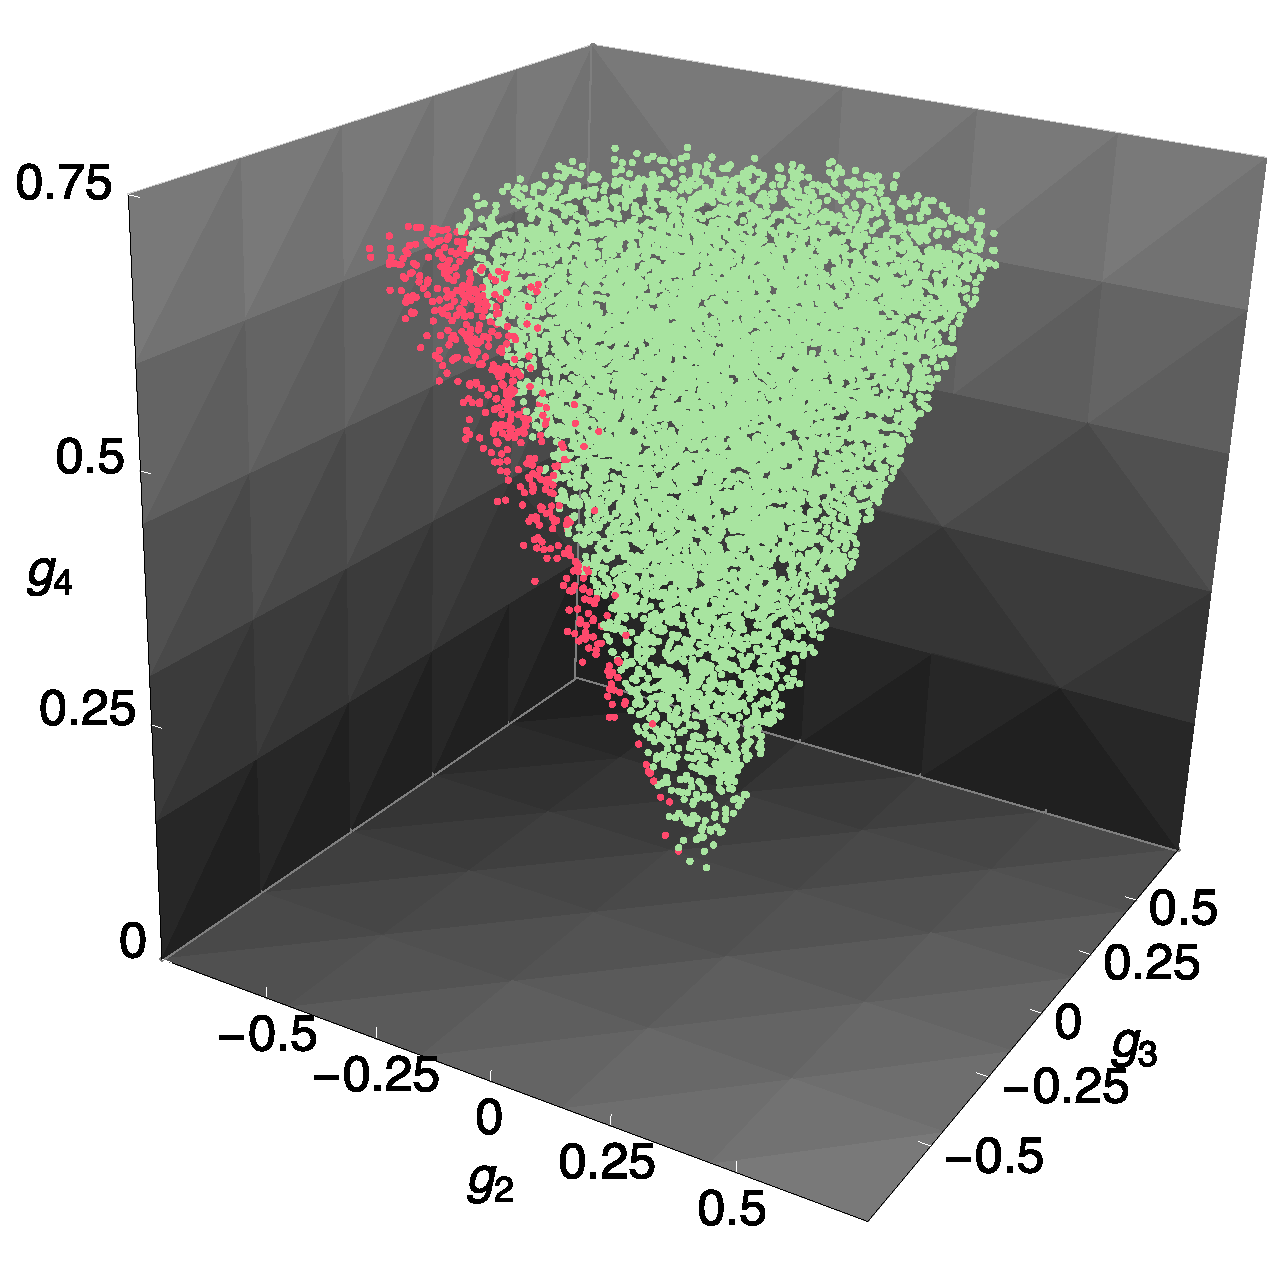
\includegraphics[width=\columnwidth]{g3Dplot.eps}
\caption{
Same as Fig.~\ref{fig:c3Dplot}, except the coordinates have been transformed
from $\{c_2,c_3,c_4\}\to\{g_2,g_3,g_4\}$. In this parametrization, the green 
points are well described by a cone of radius, $R=1/2$ and height, 
$H=(-4 + 10\sqrt{2}/3)$.
}
\label{fig:g3Dplot}
\end{figure}

\subsection{Sampling from the Conal Region}

The samples shown in Fig.~\ref{fig:g3Dplot} appear consistent with points
uniformly drawn from within the volume of a cone. We here describe the
mathematical formalism by which one can compute such samples.

Samples may be drawn from a cone by first considering how to draw samples
uniformly from within a circle. This well-known problem can be tackled by
using polar co-ordinates and drawing a random polar angle $\theta$ in the range
$0$ to $2\pi$ radians and a random radius $r$ from a triangular distribution
between $0$ and $\rho$, where $\rho$ is the full radius. We now note that the
radius varies as a function of height, $h$, along the cone, such that 
$\rho(h) = R h/H$. Finally, $h$ is drawn from a quadratic power law
distribution from $0$ to $H$ (the full height), since the area of a circle 
increases as $\rho^2$. Drawing a random uniform variate for $\alpha_{\theta}$,
$\alpha_h$ and $\alpha_r$ between 0 and 1, the polar angles, height and radius
of a point uniformly drawn from within the cone may be expressed as:

\begin{align}
\theta &= 2 \pi \alpha_{\theta},\\
h &= H \alpha_h^{1/3},\\
r &= \frac{ R h \sqrt{\alpha_r} }{ H }.
\end{align}

Converting these into Cartesian elements, we have:

\begin{align}
g_2 &= r \sin \theta,\\
g_3 &= r \cos \theta,\\
g_4 &= h.
\end{align}

Or more explicitly:

\begin{align}
g_2 &= R \alpha_h^{1/3} \alpha_r^{1/2} \sin ( 2 \pi \alpha_{\theta} ),\\
g_3 &= R \alpha_h^{1/3} \alpha_r^{1/2} \cos ( 2 \pi \alpha_{\theta} ),\\
g_4 &= H \alpha_h^{1/3} .
\end{align}

We may also express the $c_i$ coefficients in terms of the uniform random
variates, $\alpha_i$:

\begin{align}
c_2 =& \frac{\alpha_h^{1/3}}{12} \Bigg( 28 (9-5\sqrt{2}) \nonumber\\
\qquad& + 3 \alpha_r^{1/2} \Big( -6\cos(2\pi\alpha_{\theta}) 
+ (3+10\sqrt{2}\sin(2\pi\alpha_{\theta}) \Big) \Bigg),\\
c_3 =& \frac{\alpha_h^{1/3}}{9} \Bigg( -632 + 396 \sqrt{2} \nonumber\\
\qquad& + 3\alpha_r^{1/2}(4-21\sqrt{2})\sin(2\pi\alpha_{\theta}) \Bigg) ,\\
c_4 =& \frac{\alpha_h^{1/3}}{12} \Bigg( 28 (9-5\sqrt{2}) \nonumber\\
\qquad& + 3 \alpha_r^{1/2} \Big( 6\cos(2\pi\alpha_{\theta}) 
+ (3+10\sqrt{2}\sin(2\pi\alpha_{\theta}) \Big) \Bigg).
\label{eqn:alpha}
\end{align}

One may now work in the $\boldalpha$ parameter space, drawing samples from 
within a unit cube and then converting into a physically plausible set of LDCs
using the above.

A unique set of inverse relations can be defined by use of an arc tangent
accounting for the quadrant of the radical and the use of a floor function.
We have written Python and Fortran code, called \LDC, to perform
these functions, which is publicly available at \link.

\subsection{Testing Samples Drawn from the Conal Region}

We have provided no formal proof that the loci of points in $g$-space is bound
by a cone, nor do we explicitly claim so. We merely observe that the morphology 
of the loci most closely resembles this shape, from which it is possible to 
easily draw uniform samples. We here provide two simple tests demonstrating that 
sampling from the conal region provides an excellent set of physical LDCs.

First, we generated $10^6$ uniform random points from within the cone and 
tested whether they satisfied the physical conditions \I, \II\ and \III. 
Using $R=1/2$ and $H=(-4 + 10\sqrt{2}/3)$, we find that 97.3\% of the conal
region is physical, or equivalently, points sampled from this region have a 
validity of 97.3\%. Similarly, using the sample of $10^4$ valid points generated 
earlier in \S\ref{sub:validitytests}, we find a completeness of 94.4\%. 
Therefore, points samples from the conal region crop $\sim5$\% of the allowed 
parameter space.

%%% 3D plot of the alpha-space
\begin{figure}
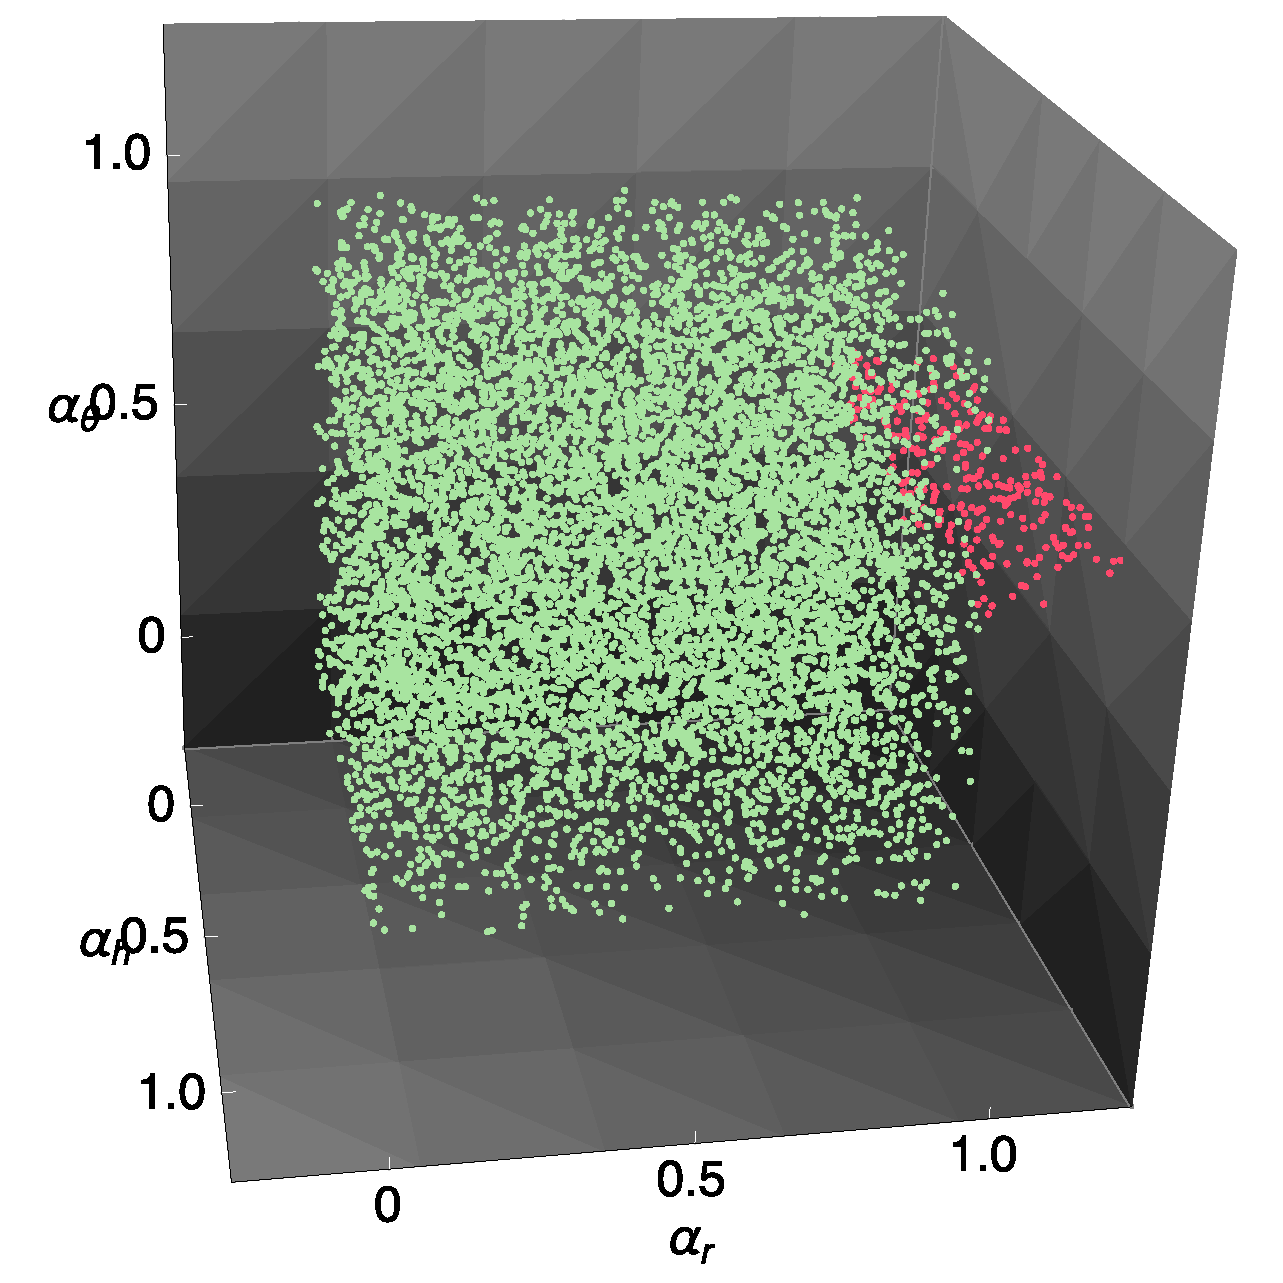
\includegraphics[width=\columnwidth]{alpha3Dplot.eps}
\caption{
Same as Fig.~\ref{fig:c3Dplot}, except the coordinates have been transformed
from $\{c_2,c_3,c_4\}\to\{\alpha_h,\alpha_r,\alpha_{\theta}\}$. In this 
parametrization, the green points are nearly uniformly distributed within a
unit cube. One may therefore uniformly sample from the cube in 
$\boldalpha$-space and then transform back to $\mathbf{c}$-space to efficiently
sample physical LDCs.
}
\label{fig:alpha3Dplot}
\end{figure}

Aside from validity and completeness, we also consider the distribution of LDCs
generated from sampling the conal region. We find that uniform samples from the
$\mathbf{g}$-cone (or equivalently uniform points in the $\boldalpha$-cube)
yield $\{c_2,c_3,c_4\}$ LDCs closely matching the distribution which would
result from uniform sampling in $\mathbf{c}$-space with a simple 
acceptance/rejection of criteria A-G. This is evident in 
Fig.~\ref{fig:chistos}, where we compare the nearly identical distributions 
from these two approaches. One can also see in Fig.~\ref{fig:alpha3Dplot}, 
that the valid samples plotted in $\boldalpha$-space (which were initially drawn 
uniformly in $\mathbf{c}$-space) provide an approximately uniform set of points 
within the unit cube.

%%% Histograms of conally simulated LDCs (in c-space)
\begin{figure}
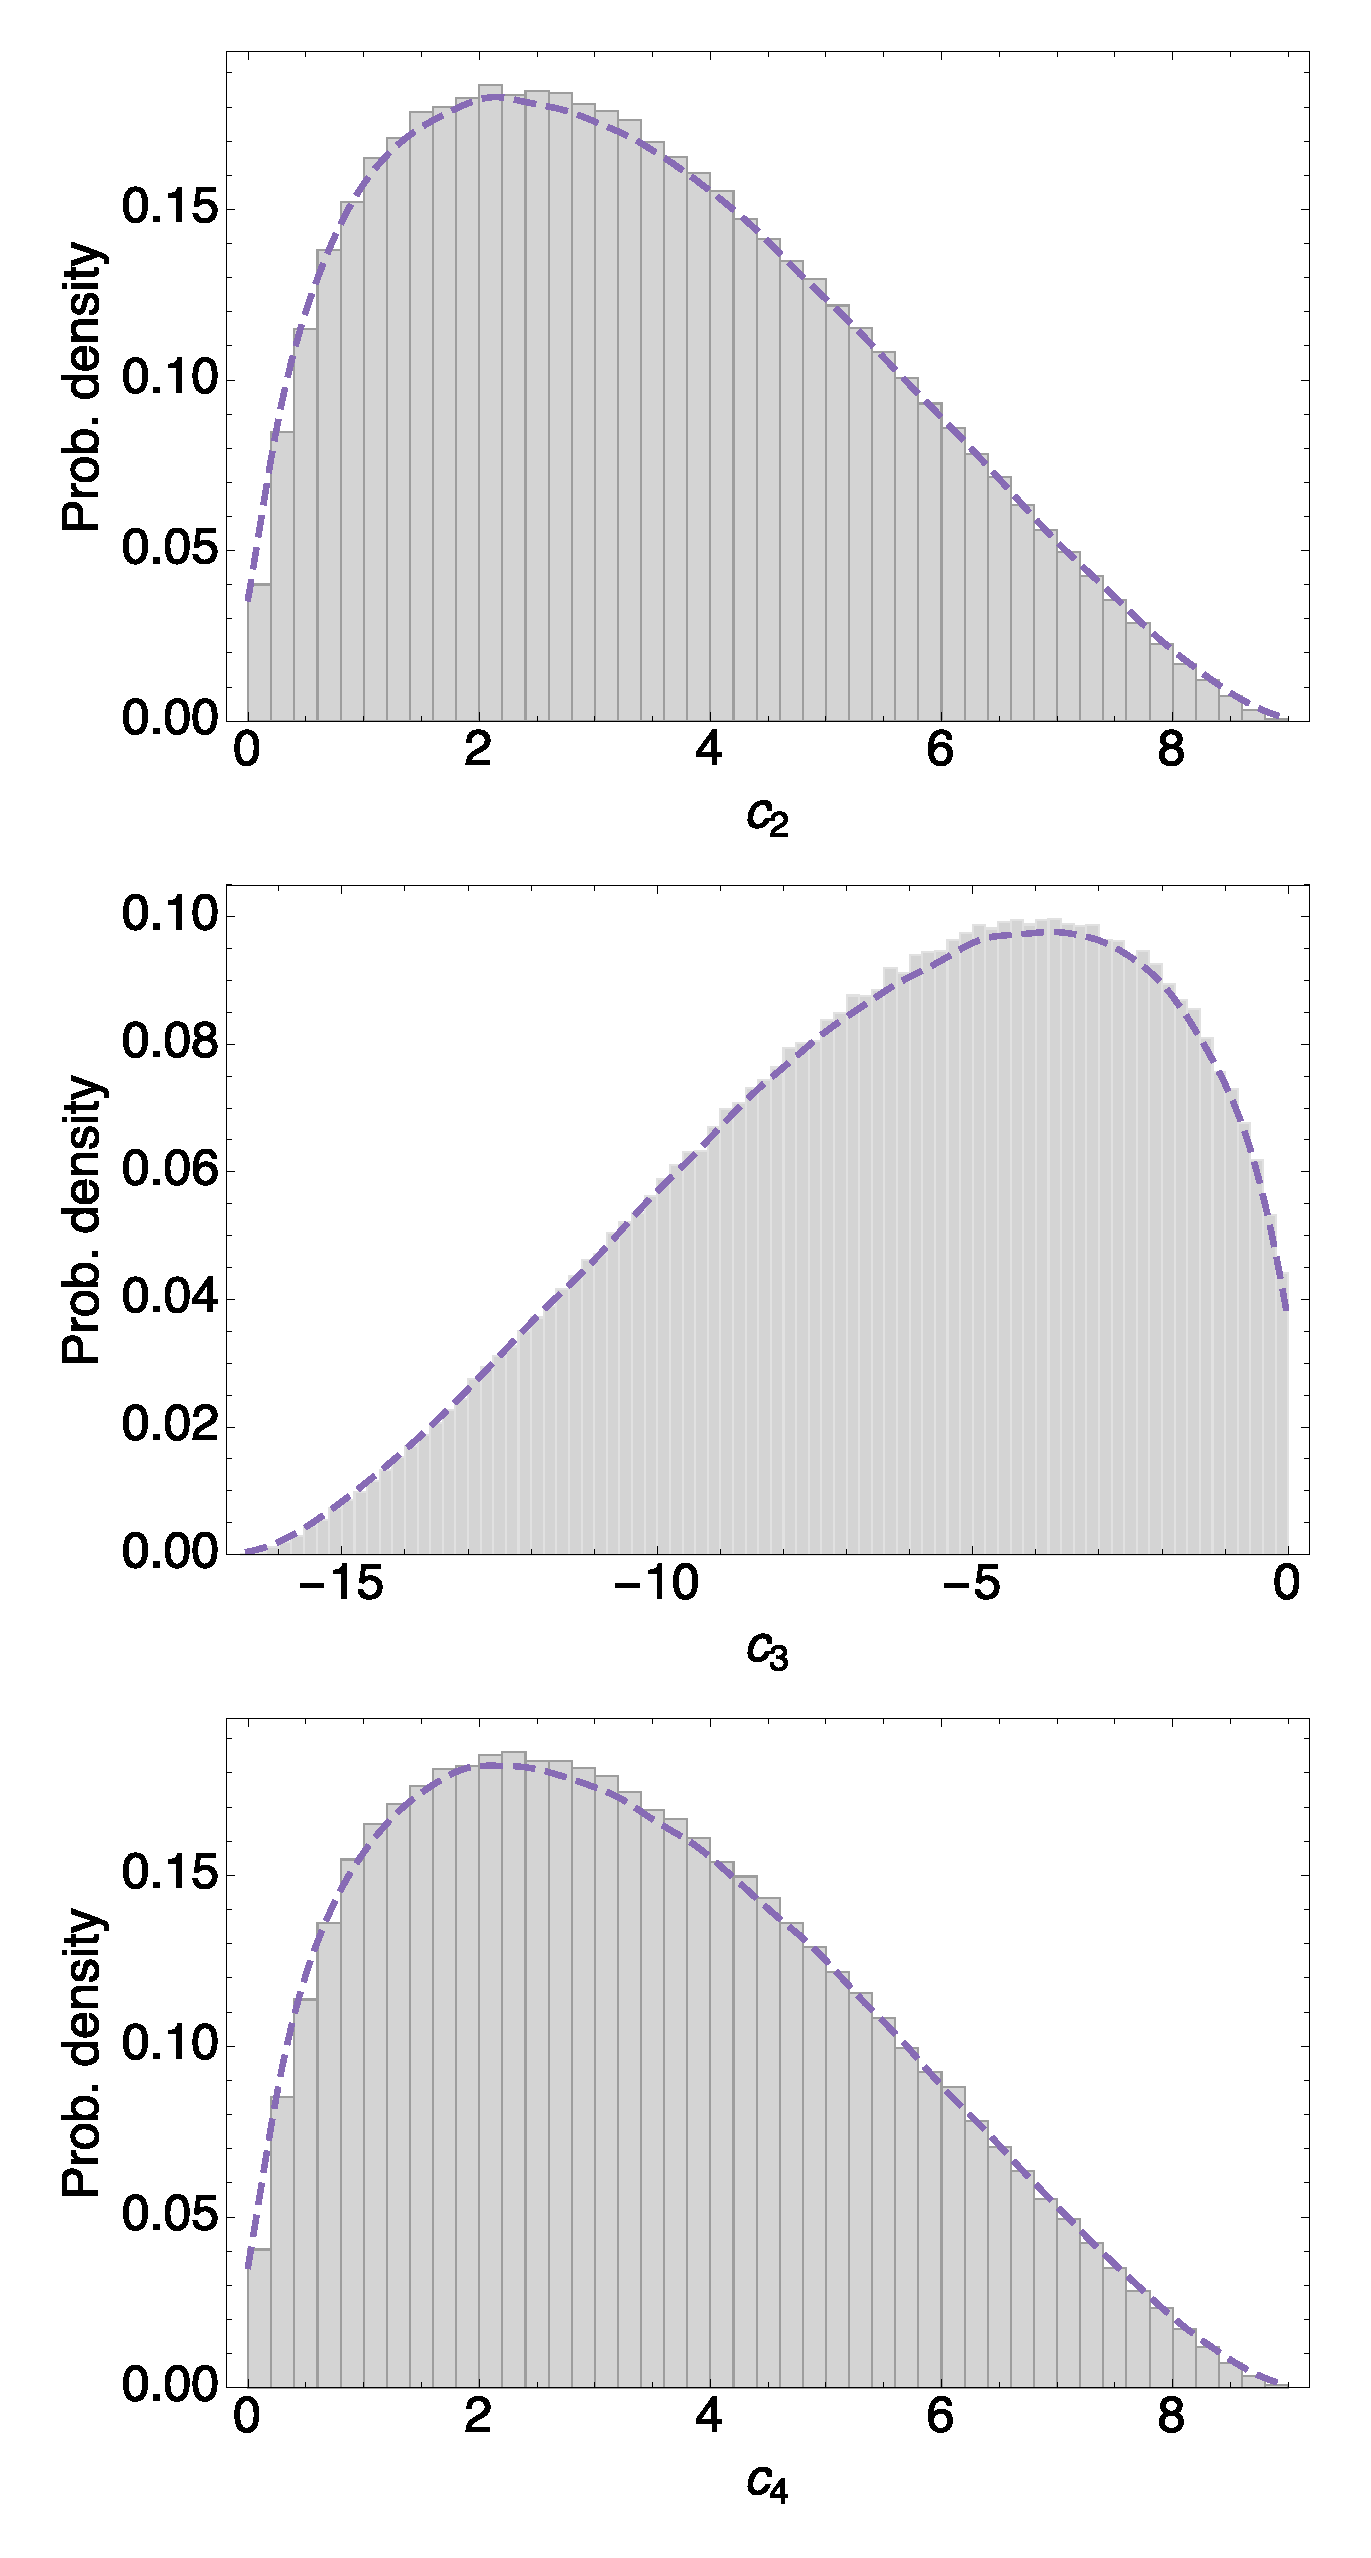
\includegraphics[width=\columnwidth]{chistos.eps}
\caption{
Dashed, purple lines depict smoothed histograms of $10^6$ LDCs generated by 
uniformly sampling from the conal region and then transforming from $\boldalpha 
\to \mathbf{c}$ parameter space. Gray histograms depict $10^6$ LDCs drawn from a 
random uniform prior in $\mathbf{c}$ parameter space which also satisfy the 
seven analytic criteria. The close agreement demonstrates the effectiveness of 
directly sampling from the conal region to draw physical LDCs.
}
\label{fig:chistos}
\end{figure}
